\documentclass[noheader]{coursclass}

\usetikzlibrary{calc,positioning}

\begin{document}

\vspace*{-1.5cm}
\begin{definition}[Arbre de probabilités]
	Une expérience aléatoire peut être représentée par un \textbf{arbre de probabilités} si elle est composée de plusieurs \textbf{épreuves} qui se suivent.
\end{definition}

\begin{exemple}
	\begin{minipage}{0.4\linewidth}
		On fait une expérience qui consiste à :
		\begin{itemize}
			\item Lancer une pièce à pile ou face
			\item Lancer un dé équilibré, et regarder si on a fait un $6$.
		\end{itemize}
	\end{minipage}
	\begin{minipage}{0.55\linewidth}
		\begin{center}
			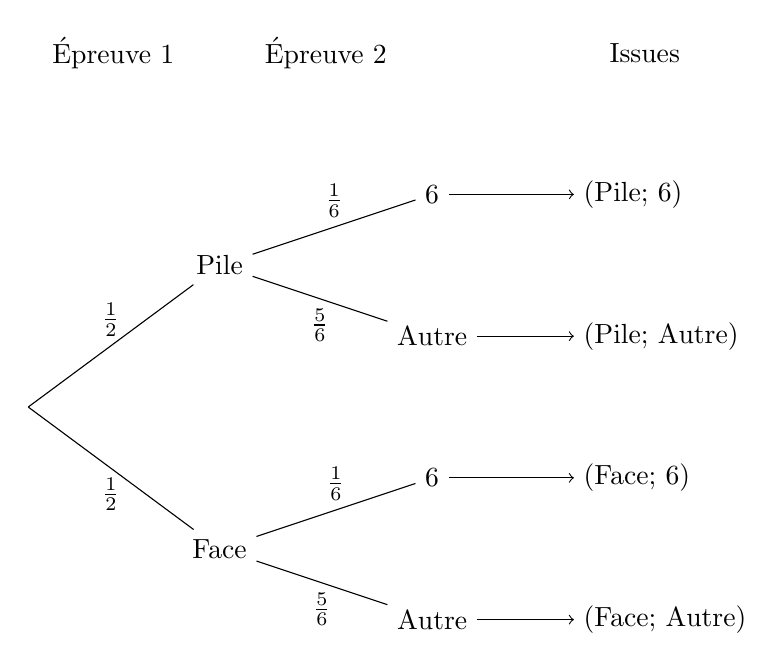
\begin{tikzpicture}[scale=0.9]
				\coordinate (START) at (0.3,0);

				\node at (1.5,5) {Épreuve 1};
				\node at (4.5,5) {Épreuve 2};
				\node at (9,5) {Issues};

				\node (Pile) at (3,2) {Pile};
				\node (Face) at (3,-2) {Face};
				\draw (START) -- node[above] {$\frac{1}{2}$} (Pile)
				(START) -- node[below] {$\frac{1}{2}$} (Face);
				\foreach \n in {Pile,Face} {
						\node (Ab) at ($(\n) + (3,1)$) {$6$};
						\node (NAb) at ($(\n) + (3,-1)$) {Autre};
						\draw (\n) -- node[above] {$\frac{1}{6}$} (Ab);
						\draw (\n) -- node[below] {$\frac{5}{6}$} (NAb);

						\draw[->] (Ab) -- ++(2,0) node[right] {\correction{(\n ; $6$)}};
						\draw[->] (NAb) -- ++(2,0) node[right] {\correction{(\n ; Autre)}};
					}
			\end{tikzpicture}
		\end{center}
	\end{minipage}
\end{exemple}

\begin{propriete}
	Pour obtenir la probabilité d'une issue, on \textbf{multiplie} les probabilités sur les branches menant à cette issue.
\end{propriete}

\begin{exemple}
	Sur l'exemple ci-dessus les probabilités sont :
	\begin{itemize}
		\item (Pile ; $6$) → \correctionDots{$\dfrac{1}{2} × \dfrac{1}{6} = \dfrac{1}{12}$}
		\item (Pile ; Autre) → \correctionDots{$\dfrac{1}{2} × \dfrac{5}{6} = \dfrac{5}{12}$}
		\item (Face ; $6$) → \correctionDots{$\dfrac{1}{2} × \dfrac{1}{6} = \dfrac{1}{12}$}
		\item (Face ; Autre) → \correctionDots{$\dfrac{1}{2} × \dfrac{5}{6} = \dfrac{5}{12}$}
	\end{itemize}
\end{exemple}

\begin{propriete}
	Pour obtenir la probabilité d'un évènement, on \textbf{additionne} les probabilités des issues qui le constitue.
\end{propriete}

\begin{exemple}
	Si on cherche la probabilité de l'évènement «On a fait face OU on a fait un $6$», les issues \ (Pile ; $6$), (Face ; $6$) ou (Face ; Autre) conviennent.

	La probabilité de cet évènement est donc \correctionDots{$\dfrac{1}{12} + \dfrac{1}{12} + \dfrac{5}{12} = \dfrac{7}{12}$}
\end{exemple}

\end{document}